\chapter{HASIL DAN PEMBAHASAN}
\label{hasil-dan-pembahasan}
Bangunan yang dijadikan objek penelitian adalah \textit{climate chamber} DTNTF FT UGM. Dalam bab ini, akan dibahas mengenai hasil rancang bangun sistem kendali sesuai dengan langkah-langkah yang dijelaskan pada Bab IV dengan memvariasikan berbagai macam masukan, kemudian mengetahui keluarannya. Variasi masukan dan keluaran akan dimodelkan dengan model jaringan saraf tiruan untuk mendapatkan parameter-parameter model yang dapat mengendalikan sistem bangunan.

\section{Hasil Pengambilan Data Simulasi IES-VE}

\subsection{Kondisi \textit{Climate Chamber}}
\begin{figure}[!h]
	\centering
	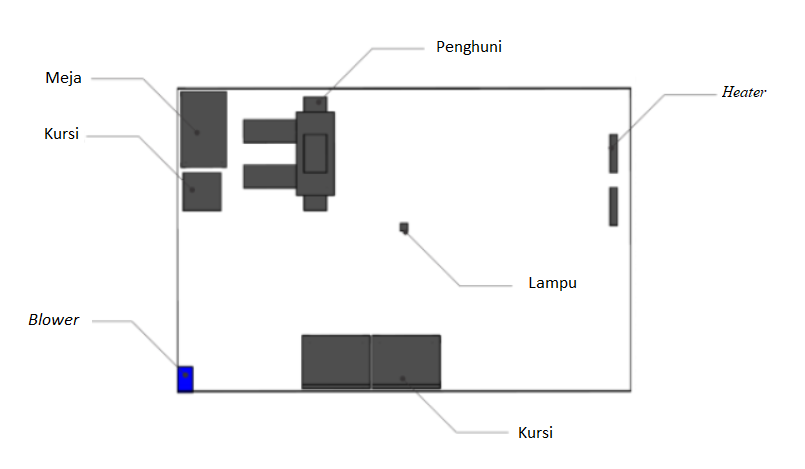
\includegraphics[width=1\textwidth]{figures/KondisiChamber}
	\caption{Posisi Komponen \textit{Climate Chamber}}
	\label{fig:5:KondisiChamber}
\end{figure}

\textit{Climate chamber} pada penelitian ini memiliki ukuran $3m \times 2m \times 3m$ ($p \times l \times t$). Komponen-komponen di dalam \textit{climate chamber} terdiri dari meja, kursi, \textit{blower}, penghuni, lampu, \textit{heater}, dan AC. 

\begin{figure}[h]
	\centering
	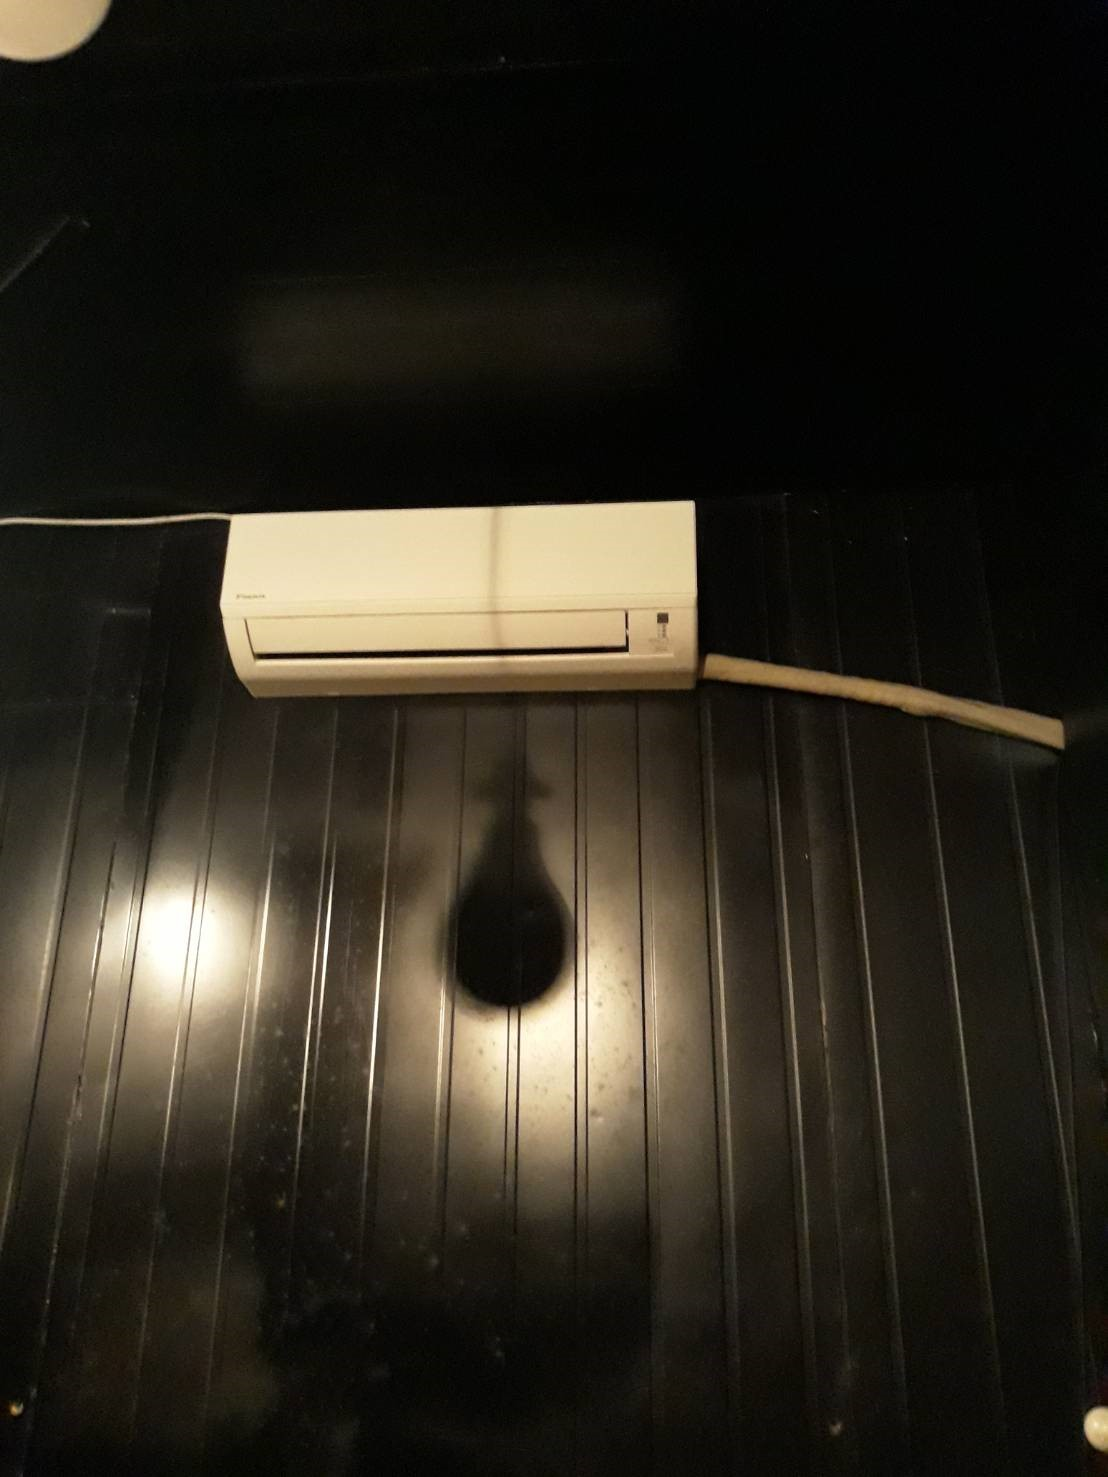
\includegraphics[width=0.5\textwidth]{figures/AC}
	\caption{Perangkat AC}
	\label{fig:5:AC}
\end{figure}

Gambar \ref{fig:5:AC} adalah AC yang berada di dalam \textit{climate Chamber} DTNTF UGM. AC yang digunakan pada \textit{climate chamber} memiliki daya sebesar 2800 W (1 PK). Secara keseluruhan pengaruh AC pada \textit{climate chamber} sangat berpengaruh dalam membentuk kondisi lingkungan termal. Hal ini dikarenakan kemampuan AC yang mampu mengkondisikan lingkungan termal sesuai dengan \textit{set point}.

\begin{figure}[h]
	\centering
	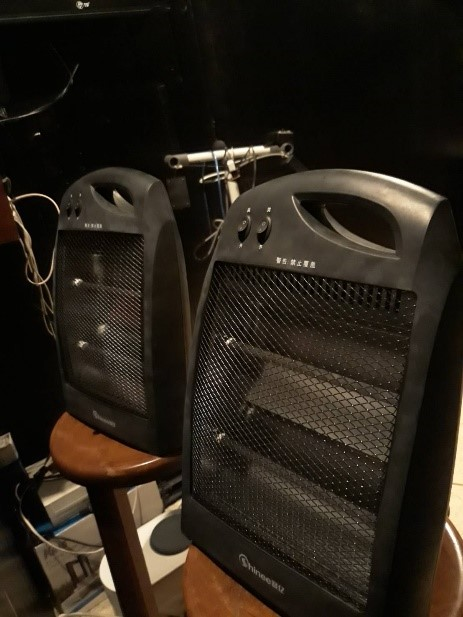
\includegraphics[width=0.5\textwidth]{figures/Heater}
	\caption{Perangkat \textit{Heater}}
	\label{fig:5:Heater}
\end{figure}

Gambar \ref{fig:5:Heater} adalah \textit{heater} yang berada di dalam \textit{climate chamber} DTNTF UGM. Heater yang digunakan pada studi kasus penelitian ini memiliki daya sebesar 900W. Semakin banyak heater yang aktif maka akan semakin meningkat suhu udara pada \textit{climate chamber}. Kenaikan rerata akibat adanya sebesar $\pm$1,9$^{\circ}$C untuk setiap heater.

\begin{table}[hbt!]
	\caption{U-Value Selubung \textit{Climate Chamber}}
	\label{tbl:5:UValue}
	\centering
	% use packages: array
	\begin{tabular}{|l|l|}
		\hline
		\textbf{Selubung \textit{climate chamber}} & \textbf{U-Value (W/m$^2$.K)} \\ \hline
		Dinding & 0,707 \\ \hline
		Lantai  & 1,996 \\ \hline
		Atap    & 0,707 \\ \hline
	\end{tabular}
\end{table}

\subsection{Hasil Rancangan Skenario}
\begin{figure}[h]
	\centering
	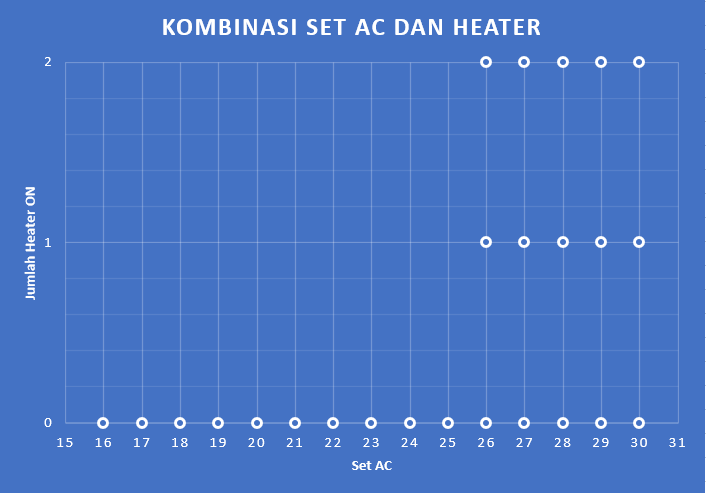
\includegraphics[width=0.8\textwidth]{figures/HeaterAC}
	\caption{Skenario Set Suhu AC dan Jumlah Heater ON}
	\label{fig:5:HeaterAC}
\end{figure}
Kombinasi antara jumlah \textit{heater} ON dan Set AC terdapat 25 skenario. Untuk variasi suhu lingkungan dan radiasi matahari dipilih 4 titik ekstrim bumi terhadap matahari yaitu pada 21 Maret, 21 Juni, 23 September dan 22 Desember. Setiap titik tersebut dilakukan simulasi dengan kombinasi heater dan AC seperti pada Gambar \ref{fig:5:HeaterAC}. Jadi total skenario yang dihasilkan dari kombinasi tersebut terdapat 100 skenario.

\subsection{Hasil Simulasi IES-VE}

\section{Pembangunan Arsitektur JST}
Data dibagi menjadi 3 bagian, yakni 70\% data pelatihan, 15\% data validasi, dan 15\% data pengujian. Model JST menggunakan arsitektur \textit{multilayer perceptron} dengan jumlah neuron sebanyak $x_1$ di lapisan tersembunyi 1, $x_2$ di lapisan tersembunyi 2, dan $x_3$ di lapisan tersembunyi 3.

\section{Analisis Kinerja Arsitektur JST yang terpilih}

Persamaan ditulis rata tengah dan nomor persamaan ditulis rata kanan. Nomor persamaan
diurutkan dengan format (nomor\_bab.nomor\_persamaan). Contoh dapat dilihat pada Persamaan \eqref{eq:1}.

\begin{equation}
    \dfrac{Dv}{Dt} = \dfrac{\partial v}{\partial t} + \nabla \cdot \mathbf{uu}
\label{eq:1}
\end{equation}

